% SEGMENT OLP-0050-S01
% Part: sets-functions-relations
% Chapter: infinite
% Section: hilberts-hotel
%
\documentclass[../../../include/open-logic-section]{subfiles}

\begin{document}

\olfileid{sfr}{infinite}{hilbert}
\olsection{ஹில்பர்ட்டின் விடுதி}

இயல் எண்களின் கணம் முடிவுறாதது என்பது தெளிவு.
எனவே இயல் எண்களை \emph{முன்கொள்ள} விரும்பவில்லை எனில்,
இயல் எண்களையே குறிப்பிடத் தேவையில்லாத சொற்களைக் கொண்டு
ஒரு முடிவுறாத கணத்தைப் பண்புரைப்பதே நமது முதல் படியாக இருக்க வேண்டும்.
1924ஆம் ஆண்டுச் சொற்பொழிவு ஒன்றில் ஹில்பர்ட் முன்வைத்த நேர்த்தியான
ஓர் அணுகுமுறை இதோ. பின்வருமாறு கற்பனை செய்யுமாறு அவர் கேட்கிறார்:
\begin{quote}
[\ldots] முடிவுறு எண்ணிக்கையிலான அறைகளைக் கொண்ட ஒரு விடுதி.
இந்த அறைகள் ஒவ்வொன்றிலும் சரியாக ஒரு விருந்தினர் தங்கியிருக்க வேண்டும்.
இப்போது விருந்தினர்கள் தங்கள் அறைகளை ஏதாவது ஒரு வகையில் மாற்றிக்கொண்டு,
[ஆனால்] ஒவ்வோர் அறையிலும் இன்னும் அதிகபட்சம் ஒருவரே இருக்குமாறு செய்தால்,
எந்த அறையும் காலியாகாது; இவ்வாறு விடுதி உரிமையாளரால் புதிதாக வரும்
விருந்தினருக்கு ஒரு புதிய இடத்தை உருவாக்க முடியாது [\ldots
\textparagraph \ldots]

இப்போது விடுதியில் $1$, $2$, $3$, $4$, $5$, \dots என்று
எண்களிடப்பட்ட முடிவுறாத எண்ணிக்கையிலான அறைகள் இருக்கட்டும்;
ஒவ்வொன்றிலும் சரியாக ஒரு விருந்தினர் தங்கியிருக்கிறார்.
ஒரு புதிய விருந்தினர் வந்தவுடன், பழைய விருந்தினர்கள் ஒவ்வொருவரையும்
அவர்களது அறை எண்ணைவிட ஒன்று அதிகமான எண்ணுடைய அறைக்கு உரிமையாளர்
மாற்றினால் போதும்; புதிதாக வரும் விருந்தினருக்காக அறை~$1$ காலியாகும்.
	\begin{center}
		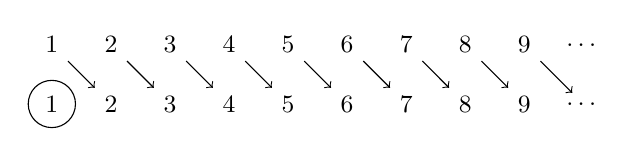
\begin{tikzpicture}[scale = .75]
		\foreach \x in {1, 2, 3, 4, 5, 6, 7, 8, 9}
		{
			\node (\x a) at (\x, 1) {\small{\x}};
			\node (\x b) at (\x, 2) {\small{\x}};
		}
		\node (dotsa) at (10, 1) {\small{\ldots}};
		\node (dotsb) at (10, 2) {\small{\ldots}};
		\draw[->] (1b)--(2a);
		\draw[->] (2b)--(3a);
		\draw[->] (3b)--(4a);
		\draw[->] (4b)--(5a);
		\draw[->] (5b)--(6a);
		\draw[->] (6b)--(7a);
		\draw[->] (7b)--(8a);
		\draw[->] (8b)--(9a);
		\draw[->] (9b)--(dotsa);
		\draw (1,1) circle (.4);
		\end{tikzpicture}
	\end{center}
	(\citealt[730]{EwaldSieg2013} இல் வெளியிடப்பட்டது;
    OpenLogic ஆசிரியர்களின் மொழிபெயர்ப்பு)
\end{quote}

% SEGMENT OLP-0050-S02
ஹில்பர்ட்டின் விடுதியில் முடிவுறாத எண்ணிக்கையிலான அறைகள் உள்ளன
என்பதே முக்கியக் கருத்து; அவ்வாறு கூறுவதன் பொருளை வரையறுப்பதாக
அவரது விளக்கத்தை எடுத்துக்கொள்ளலாம்.
உண்மையில் இதுவே டெடெகிண்டின் அணுகுமுறை
(நிச்சயமாக, இங்கு பெரும் காலப்பொருத்தமின்மையுடன் வழங்கப்பட்டுள்ளது;
டெடெகிண்டின் வரையறை \citeyear{Dedekind1888} ஆண்டைச் சேர்ந்தது):

% SEGMENT OLP-0050-S03
\begin{defn}\ollabel{defn:DedekindInfinite}
$A$ இலிருந்து $A$ இன் ஒரு தகு உட்கணத்திற்குச் செல்லும்
!!a{injection} இருக்கும்போது, அப்போதும் அப்போது மட்டுமே,
ஒரு கணம் $A$ என்பது \emph{டெடெகிண்ட்-முடிவுறாதது} ஆகும்.
அதாவது, $o \notin \ran{f}$ என அமையும் ஏதோ ஒரு $o \in A$ உம்
!!a{injection} $f \colon A \to A$ உம் உள்ளன.
\end{defn}

\end{document}
